\documentclass[a4paper,12pt]{article}

% packages
\usepackage{amsmath}
\usepackage{amssymb}
\usepackage{graphicx}
\usepackage{fancyhdr}
\usepackage{hyperref}
\usepackage{float}



% Fancy header/footer settings
\pagestyle{fancy}
\fancyfoot[C]{}
\fancyfoot[R]{\thepage} % Right-align page number in the footer


% Title information
\title{AAD - Assignment 2}
\author{107474-Joseane Pereira \\
109050-Gabriel Costa \\
Universidade de Aveiro, DETI}
\date{\today}

\begin{document}

\begin{figure}
    \centering
    
\includegraphics[width=0.3\linewidth]{ua.pdf}
    \label{fig:enter-label}
\end{figure}
\maketitle
\newpage
\tableofcontents
\newpage
\section{Introduction}
This assignment focuses on the implementation and analysis of different 
accumulator designs in VHDL, including a single-cycle version, a pipelined 
version, and versions with shift functionality.


\section{Implementations}
\subsection{Single-Cycle Accumulator}
As suggested with provided staring point the basic accumulator was implemented in
\texttt{accumulator\_single\_cycle.vhd} with the following features:
\begin{itemize}
    \item Simple write and read ports
    \item Direct accumulation without pipelining
    \item Basic addition functionality
\end{itemize}
\begin{figure}[H]
    \centering
    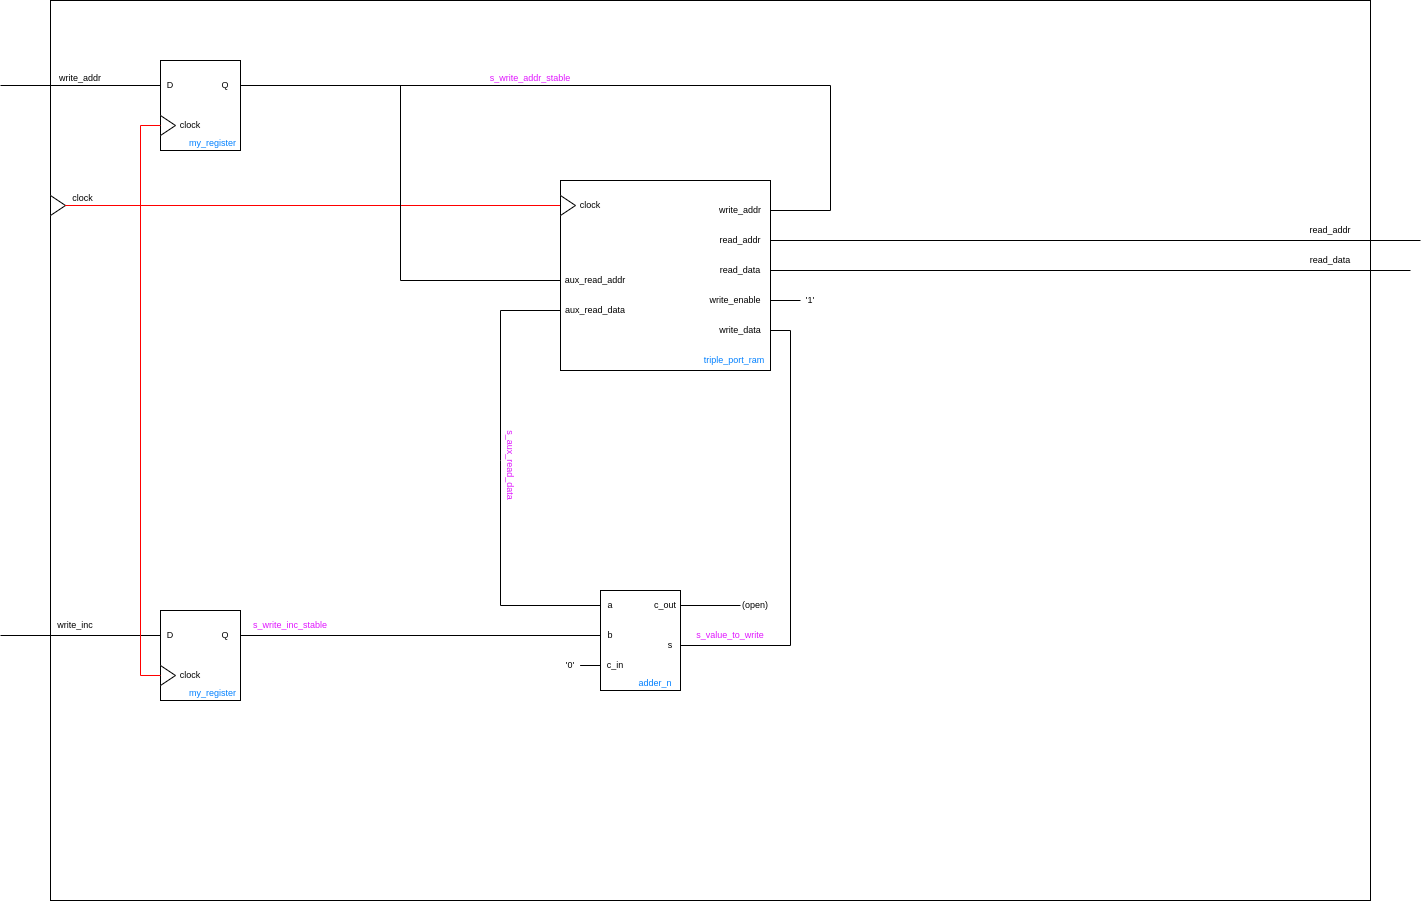
\includegraphics[width=1.0\linewidth]{accumulator_single_sycle.png}
    \caption{Single-cycle accumulator block diagram}
    \label{fig:single_cycle}
\end{figure}


\subsection{Pipelined Accumulator}
The pipelined version \texttt{accumulator\_pipeline.vhd} improves
 upon the basic design by:
\begin{itemize}
    \item Adding pipeline stages to improve throughput
    \item Using registers to stabilize signals
    \item Implementing hazard detection
\end{itemize}

\begin{figure}[H]
    \centering
    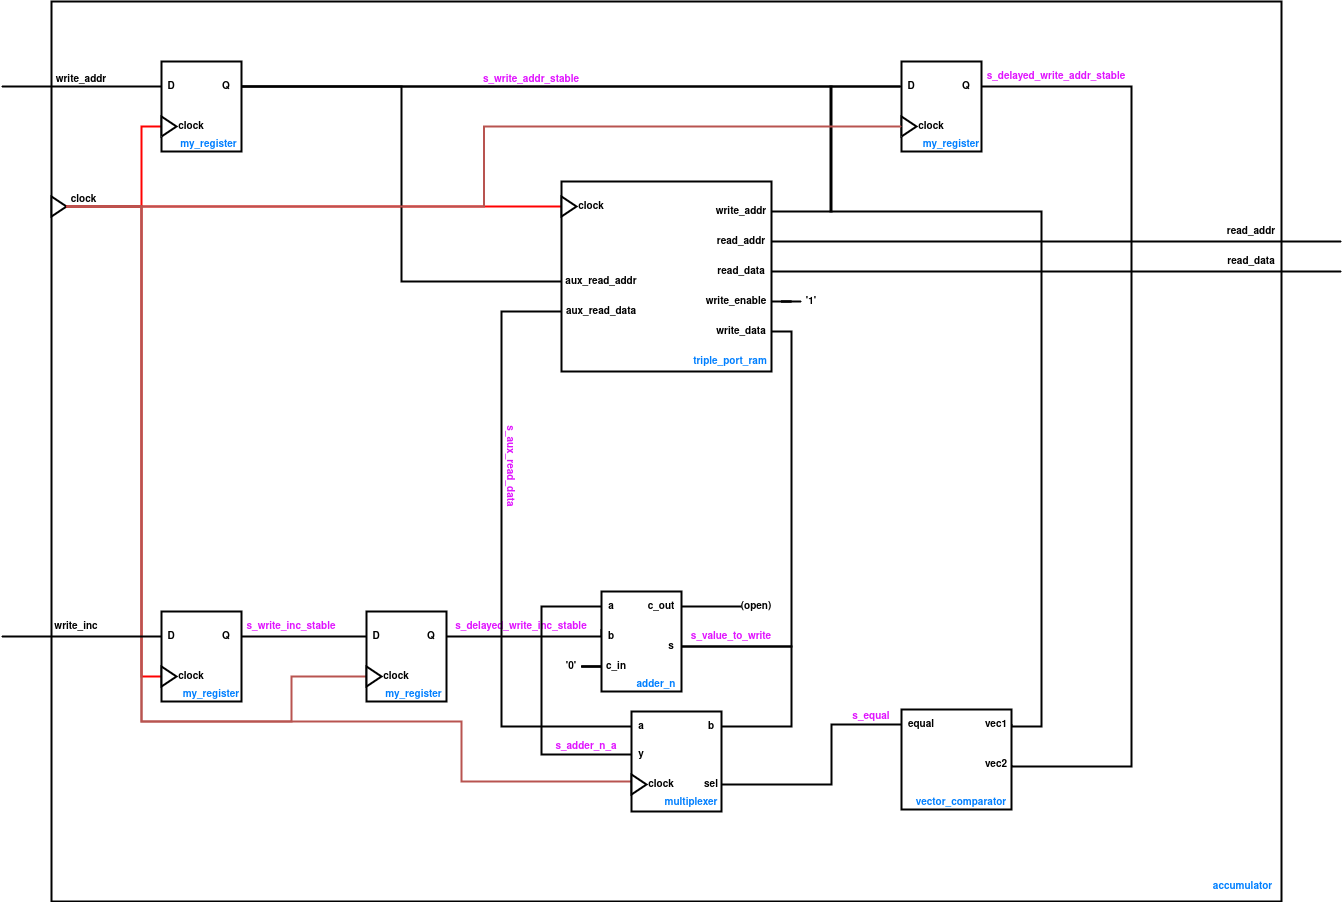
\includegraphics[width=1.0\linewidth]{accumulator_pipeline.png}
    \caption{Pipelined accumulator block diagram}
    \label{fig:pipeline}
\end{figure}

\subsection{Shift Accumulator}
We implemented a version of the accumulator using a barrel Shifter for both the pipelined and single sycle version (\texttt{shift\_accumulator\_pipeline.vhd and shift\_accumulator.vhd}) both of wich improve upon the basic design by:
\begin{itemize}
    \item Dynamic shift operations on input data
    \item Configurable shift amounts
    \item Integration with the accumulation logic
\end{itemize}

\begin{figure}[H]
    \centering
    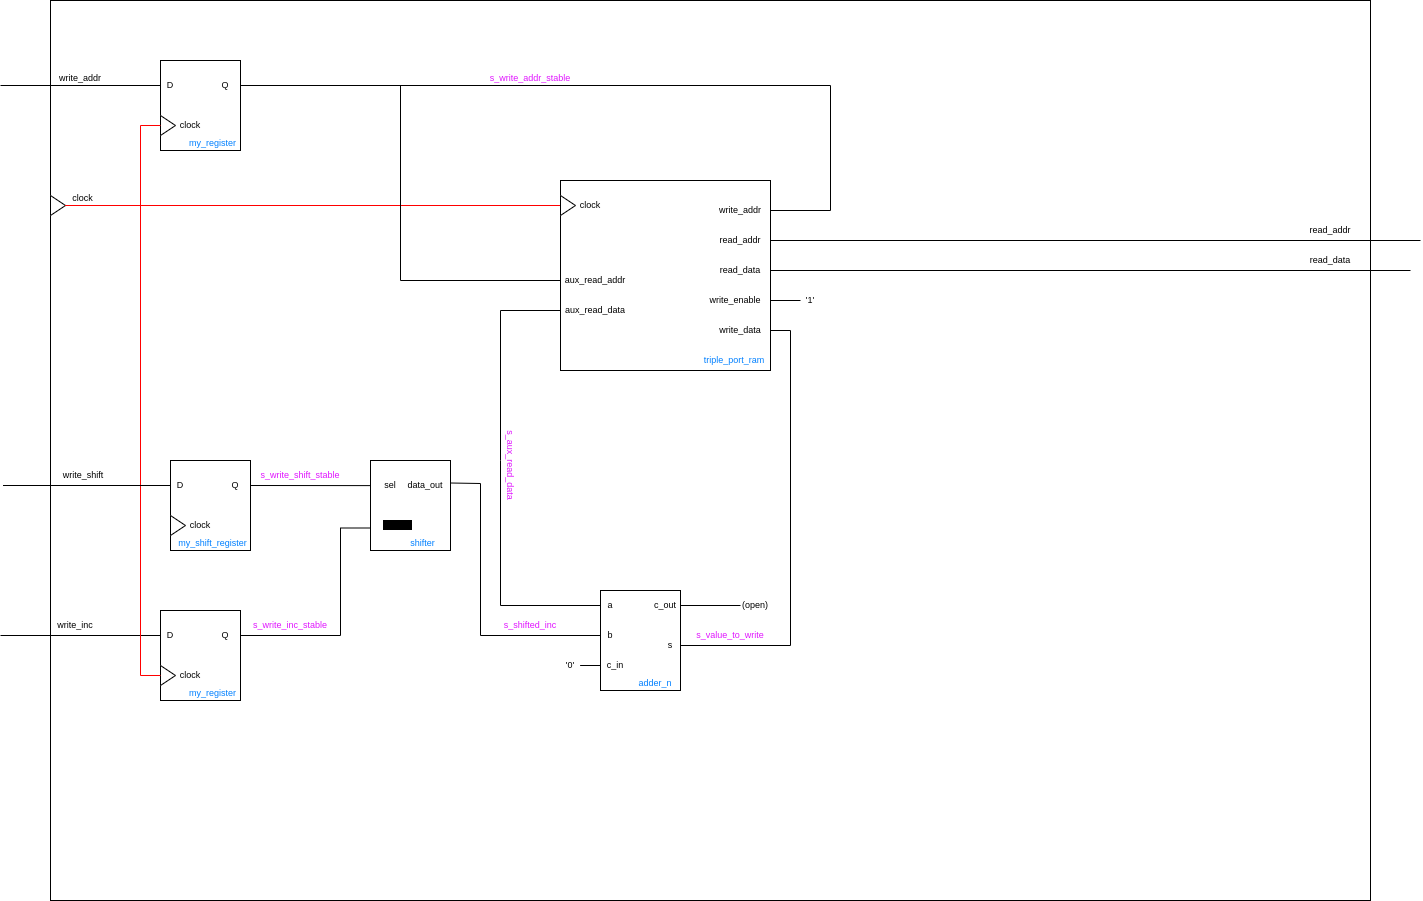
\includegraphics[width=1.0\linewidth]{accumulator_shift_single_sycle.png}
    \caption{Shift accumulator sigle sycle block diagram}
    \label{fig:shift}
\end{figure}

\begin{figure}[H]
    \centering
    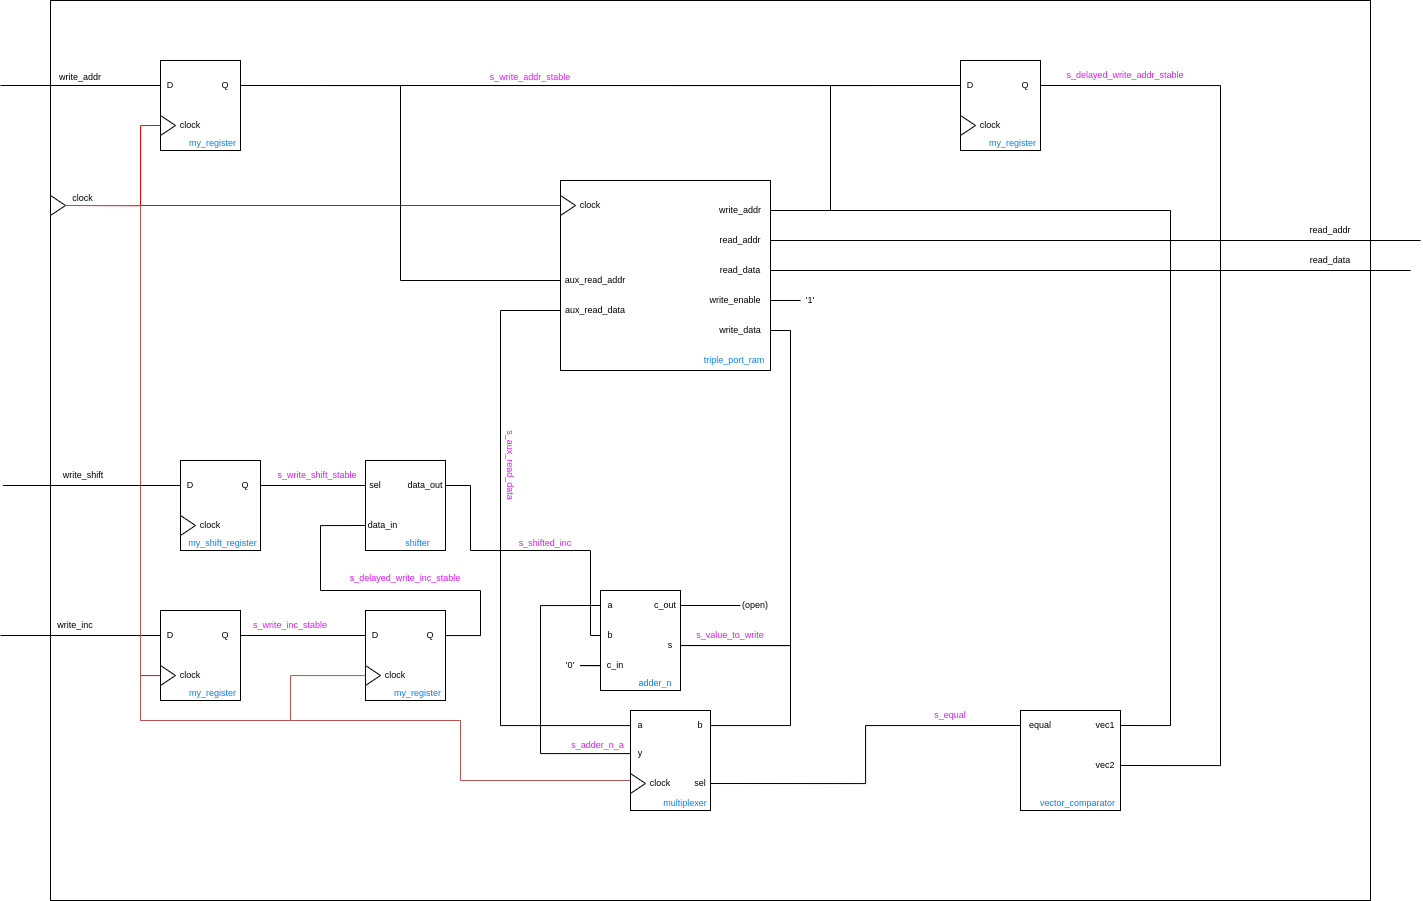
\includegraphics[width=1.0\linewidth]{accumulator_shift_pipeline.png}
    \caption{Shift accumulator pipeline block diagram}
    \label{fig:shift_pipeline}
\end{figure}


\section{Components}
Some of the Components were provided by the professor, and some were 
implemented by us.
Key components used in the designs include:
\begin{itemize}
    \item Triple Port RAM for memory storage
    \item Registers for signal stabilization
    \item Adder N for arithmetic operations
    \item Shifter for shift operations
    \item Vector Comparator for address comparison
\end{itemize}

\section{Testing}
Testing was performed using:
\begin{itemize}
    \item GHDL simulator
    \item VCD waveform generation
    \item A provisded testbench for the single-cycle accumulator adapted for the pipelined and shift versions
\end{itemize}

\section{Results and Analysis}
    % Results and analysis
    %figue waveform
\begin{figure}[H]
    \centering
    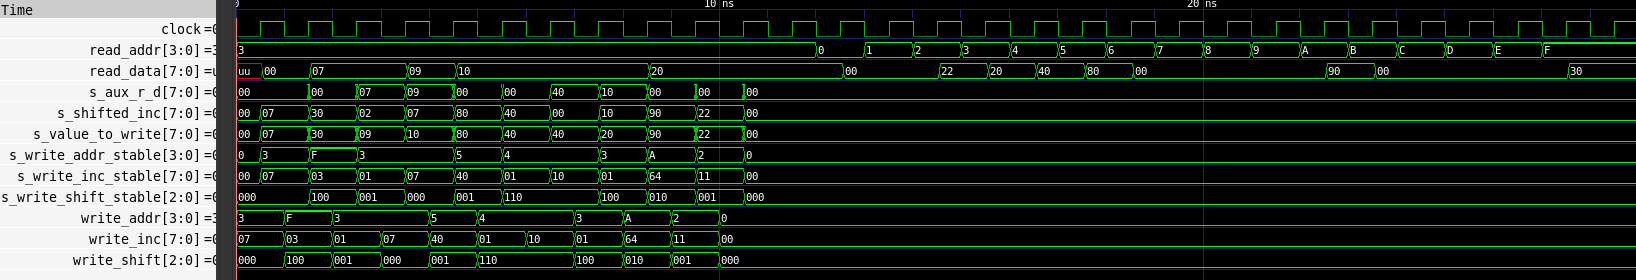
\includegraphics[width=0.8\linewidth]{waveform.png}
    \caption{Waveform of the single-cycle accumulator testbench}
    \label{fig:waveform}
\end{figure}

\ref{fig:waveform} shows the waveform generated by the testbench for the single-cycle accumulator. The testbench was adapted for the pipelined and shift versions, and the results were similar. The shift accumulator was tested with different shift amounts, and the results were as expected.

\section{Conclusions}


\end{document}